\documentclass[ddcfooter]{tudbeamer}
\usepackage{german}
\begin{document}
\title[Digital Signal Processing]{Digital Signal Processing using CUDA}
\subtitle{Digital Signal Processing using CUDA}
\author{Nico Wehmeier, Richard Pfeifer, Fabian Jung}

\maketitle

\begin{frame}
    \frametitle*{Inhalt}
    \tableofcontents[currentsection]
\end{frame}

%Verantwortlicher: ???
\section{Aufgabenstellung}
\begin{frame}
\frametitle{Aufgabenstellung}
%\framesubtitle{untertitel erste folie}
\begin{itemize} 
	\item{Ausgangsitutation}
	\begin{itemize}
		\item{Messgeräte erzeugen Datenstrom}
		\item{Datenstrom nicht kontinuierlich}
		\item{Serielle Implementierung}
	\end{itemize}
	\item{Anforderungen}
	\begin{itemize}
		\item{Portierung auf GPU}
		\item{Hoher Datendurchsatz}
		\item{Skalierbar auf bis zu 4 GPUs/Node}
	\end{itemize}
\end{itemize}
\end{frame}

%Verantwortlicher: ???
\section{Überblick}
\begin{frame}
    \frametitle*{Überblick}
	\begin{itemize}
	\item{Host}
	\begin{itemize}
		%TODO
		\item{Eingabe Datei auslesen}
		\item{Daten zwischenspeichern}
	\end{itemize}
	\item{Verwaltung Devices}
	\begin{itemize}
		\item{Daten aus Puffer lesen}
		\item{Zu den Devices streamen}
		\item{Kernel starten}
		\item{Ausgabe schreiben}
	\end{itemize}
	\item{Levenberg Marquardt}
	\begin{itemize}
		%TODO
		\item{Parameter einer Näherungsfunktion bestimmen}
		\item{Markante Stellen (Anfangs-, Endwert, Maximum) ermitteln und zurückgeben}
	\end{itemize}
	\end{itemize}
\end{frame}
%Verantwortlicher: Richard
\section{Host Code}
\begin{frame}
    \frametitle*{Host Code}
    
\end{frame}
%Verantwortlicher: Fabian
\section{Verwaltung Devices}
\begin{frame}
    \frametitle*{Verwaltung Devices}
    \begin{itemize}
    	\item{Jedes Devices wird von eigeneme Thread verwaltet}
    	\item{Asynchrone Aufrufe}
    		\itemize
    			\item{Pipeline}
    		\enditemize
    \end{itemize}
\end{frame}
\section{Levenberg Marquardt}
%Verantwortlicher: Nico
\begin{frame}
    \frametitle*{Levenberg Marquardt (1)}
    \begin{itemize}
        \item{Eingabedaten}
        	\begin{itemize}
        		\item{Samples}
	        		\begin{itemize}
	        			\item{Compute Capability 1.x: ca. 800)}
	        			\item{Compute Capability 2.0 oder höher: ca. 2500)}
	        		\end{itemize}
        		\item{Interpolationsschritt}
	        		\begin{itemize}
	        			\item{beliebige Dezimalzahl größer 0)}
	        			\item{Interpolation durch Texture Memory)}
	        		\end{itemize}
        	\end{itemize}
    \end{itemize}
\end{frame}
\begin{frame}
    \frametitle*{Levenberg Marquardt (2)}
    \begin{itemize}
        \item{Verarbeitung}
            \begin{itemize}
             	\item{eine Ausgleichungsrechnung pro Block}
             	\item{Grund: ca. das 5-fache der Sampleanzahl an Shared Memory benötigt (bei 1000 Samples ca. 20 kB)}
             	\item{Zugriff auf Samples durch Texture Memory}
	             	\begin{itemize}
	             	    \item{Shared Memory gespart}
	             	    \item{schnelle Interpolation möglich}
	             	\end{itemize}
             	\item{Vorgehensweise}
	             	\begin{itemize}
	           	        \item{Anfangs- und Endwert ermitteln}
	           	        \item{abhängig vom Schwellwert Bereich festlegen}
	           	        \item{für den Bereich Näherungsfunktion ermitteln}
	           	        \item{Qualität durch Residuen und Maximum der Funktion ermitteln}
	         	    \end{itemize}
            \end{itemize}
    \end{itemize}
\end{frame}
\begin{frame}
    \frametitle*{Levenberg Marquardt (3)}
	\begin{itemize}
        \item{Ausgabedaten}
        	\begin{itemize}
        		\item{3 Parameter einer quadratischen Funktion: $a*x^2+b*x+c$}
        		\item{Anfangs- und Endwert}
        		\item{Maximum}
        		\item{durchschnittliche Abweichung}
        		\item{Status (Fehler, Erfolg, Abbruch)}
        		
        	\end{itemize}
    \end{itemize}
\end{frame}
\begin{frame}
    \frametitle*{Levenberg Marquardt (4)}
	\begin{itemize}
        \item{Ergebnis: $fitfunktion=-0.550151*x^2+654.15509*x-203167.921875$}
        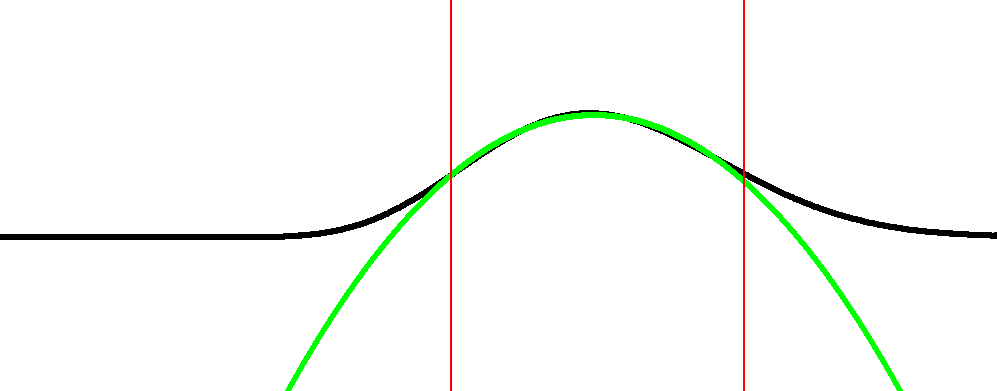
\includegraphics[height=3.5cm]{Beispielergebnis.png}
    \end{itemize}
\end{frame}
\section{Benchmark}
%Verantwortlicher: Fabian
\begin{frame}
    \frametitle*{Benchmark}
    
\end{frame}
\section{Skalierbarkeit}
%Verantwortlicher: ???
\begin{frame}
    \frametitle*{Skalierbarkeit}

\end{frame}
\section{Danksagung}

\begin{frame}
    \frametitle*{Danksagung}
    
\end{frame}
\end{document}
